\documentclass[useAMS,usenatbib,referee]{biom}
%\usepackage{authblk}
\usepackage{graphicx}
%\usepackage{subcaption}
%\usepackage{float}
\usepackage{amsmath}
%\usepackage{bm}
%\usepackage[authoryear,round, longnamesfirst]{natbib}
%\usepackage{textcomp}
%\usepackage{setspace}
%\usepackage{appendix}
%\doublespacing
%\usepackage{fancyhdr}
\usepackage[]{todonotes}
%\presetkeys{todonotes}{fancyline, color=white}{}
\usepackage{url}

%\pagestyle{fancy}
%\rhead{That's not the Mona Lisa}
%\lhead{}

%\usepackage{geometry}
%\geometry{margin=4cm}

%\usepackage{lineno}
%\linenumbers
%\linespread{1.6}

\title[How to interpret SCR density surface estimates]{That's not the Mona Lisa! How to interpret spatial capture-recapture density surface estimates}

\author{Ian Durbach$^{1,2,*}$, Rishika Chopara$^{3}$, David L. Borchers$^{1,2}$, Rachel Phillip$^{1}$, Koustubh Sharma$^{4}$ \and Ben C. Stevenson$^{3}$ \\
$^{1}$Centre for Research into Ecological and Environmental Modelling, \\ School of Mathematics and Statistics, Univeristy of St Andrews, Scotland \\
$^{2}$Centre for Statistics in Ecology, the Environment and Conservation, \\ Department of Statistical Sciences, University of Cape Town, South Africa \\
$^{3}$Department of Statistics, University of Auckland, Auckland 1010, New Zealand \\
$^{4}$Snow Leopard Trust, Seattle, Washington, United States of America \\
\email{indurbach@gmail.com}}

\begin{document}

\begin{abstract}
Spatial capture-recapture (SCR) methods are often used to estimate density surfaces, and these estimates are often misinterpreted. In particular, spatial change in density is confused with spatial change in uncertainty about where animal activity centres (ACs) are located. We illustrate correct and incorrect inference visually by treating an image of the Mona Lisa as an AC intensity surface and simulating SCR surveys from it. Inferences can be drawn about the intensity of the point process generating ACs, and about a single realisation of this process. We show that treating estimates of a realisation of the process as estimates of the intensity of the process results in invalid and misleading ecological inferences, and that estimates of the realisation are highly dependent on where the detectors are placed and how much survey effort is used. Estimates of the expected AC density surface should be obtained by estimating the intensity of a point process model for ACs. Practitioners should state explicitly whether they are estimating the intensity or the realisation, and estimates of the realisation should not be confused with the intensity of the procecss.
\end{abstract}

\begin{keywords}
Spatial capture-recapture, density surface, point processes.
\end{keywords}

\maketitle 

\section{Introduction}

Spatial capture-recapture (SCR) models \citep*{Efford:04,Borchers+Efford:08, Royle+Young:08} are now widely used to estimate animal abundance and distribution from a variety of data types, including that from camera-traps, hair snares and scat surveys, live-captures, and acoustic detectors. These methods use the location of the detectors (e.g.\ traps) and the locations at which animals were detected (their spatial capture histories) to estimate animal density. The methods have two basic components: a spatial model that quantifies animal activity centre (hereafter abbreviated to ``AC'') density at all points in the survey region, and an encounter model that quantifies the expected detection frequency or detection probability, given the AC locations and the detector locations. 

SCR density estimates are often presented graphically in the form of estimated density maps, these being easy to absorb and interpret, at least on the face of it.  However, there are various kinds of density maps that one can produce from SCR analyses and depending on what is presented, it is easy to misinterpret the maps. The most common form of misinterpretation is treating maps that include both spatially varying uncertainty about AC locations and spatially varying AC density estimates as if they were maps of AC density alone. There is also a lack of clarity about whether it is AC density or space use density that is being presented.

Examples include \cite{Dorazio+Karanth:17}, who say that such maps effectively provide  ``a species distribution model, even in cases where spatial covariates of abundance are unknown or unavailable'', \cite{Alexander+al:15}, who present a map (Figure 4) that include both spatially varying uncertainty about location and spatially varying AC density and refer to it as the ``spatial distribution of snow leopards'', and \cite{Elliot+Gopalaswamy:16}, who present the same kind of map (Figure 2) and refer to it as the ``pixel-specific lion density''. Minor variations on these themes can be found in many papers, for example ``spatial distribution of the Amur leopard density'' \citep{Qi2015}, ``a pixelated map showing fine-scale variation in density'' \citep{Fouche2020},``spatial variation in the location of estimated activity centers'' \citep{Blanc2013}, ``pixelated SPACECAP leopard density maps'' \citep{Devens2021}, ``pixel-specific densities of elephants'' \citep{Goswami2019}, ``a pixelated density map showing relative leopard density \citep{Kandel2020}, ``spatial density estimate of common leopards'' \citep{Goldberg2015}, ``density estimates in home-range centers (number of jaguars per 0.226km$^2$)'' \citep{Lavariega2020}, ``spatial patterns of dhole densities'' \citep{Srivathsa2021}, ``mean posterior density of Amur tiger'' \citep{Xiao2016}, and \cite{Chandler+Royle:13} who say ``Density surface maps can be produced by discretizing the state-space and tallying the number of activity centers occurring in each pixel during each MCMC iteration''.

The problems with interpretation of such maps arises because (a) there are various kinds of ``density'', (b) uncertainty about the locations of ACs varies spatially and this fact must be (but is often not) taken into account when interpreting estimated density surfaces from SCR surveys, and (c) there is a failure to distinguish between AC density and usage density.

We start by describing different kinds of densities involved in SCR surveys, because in any discussion of density surfaces, we need to be clear about what ``density'' means. 

\subsection{Different kinds of density}\label{different-densities}

Let us assume that ACs are generated by a Poisson process over some region of interest $\mathcal{S}$. Such a process is fully characterised by its intensity function. We could assume that the process is homogeneous, which implies ACs have a uniform distribution across the state-space. Alternatively, we can use an inhomogeneous process based on spatially referenced covariates, where the intensity at location $\bm{s}$ is given by $D(\bm{s})=\exp\left\{\beta_0 + \sum_{k=1}^K\beta_kx_k(\bm{s})\right\}$. Here, $\bm{s} \in \mathcal{S}$, $x_k(\bm{s})$ is the $k$th of $K$ spatially referenced covariates evaluated at $\bm{s}$, $\beta_0$ is an intercept parameter, and $\beta_k$ is the slope parameter for the $k$th spatially-referenced covariate. We distinguish between two kinds of spatial ``density'' below.

\subsubsection{Expected AC density surface} \label{s:eacd}

The first we call the ``expected AC density surface'', which is simply $D(\bm{s})$, the intensity function of the underlying point process that is assumed to have generated the ACs. We use the term ``expected'', because the intensity of the point process at $\bm{s}$ is approximately the expected number of ACs per unit area generated by the process in some small region surrounding $\bm{s}$ (and is exactly the expectation as the area of the region approaches zero). This quantity therefore only depends on the parameters of the point process, and is not specific to any particular realistion of points -- indeed it is an average over all possible realisations. The expected number of ACs generated by the process in any region can be calculated via integrating the intensity function, for example the expected number of activity centres in $\mathcal{S}$ is $\int_{\mathcal{S}} D(\bm{s}) \, d\bm{s}$. We can estimate the expected AC density surface by fitting a model, and plugging our estimates of $\bm{\beta}$ into the intensity
function. We denote this estimated surface as $\widehat{D}(\bm{s})$. 

%One property of a Poisson process fitted to an observed point pattern by maximum likleihood is that the estimated expected number of points is equal to $N$, the observed number of points, so that $\int_{\mathcal{S}} \widehat{D}(\bm{s}) \, d\bm{s} = N$\todo[inline]{DLB: This sentence is a bit misleading becuase we don't observe $N$, and I don't think that it necessarily integrates to $N$ when you only obsreve $n<N$ of the points? And the sentence comes out of the blue and its relevance is not clear. Seems like nothing would be lost by removing it?}

\subsubsection{Realised AC density surface} \label{s:racd}
fdsfds

\todo[inline]{dlb: After reading this subsection and suggesting some wording changes (shown below), I now think they should be ignored because I think it might be simpler/clearer if we don't talk about measurement error at all (although I know that this was my idea in the first place!). How about the text below as alternative text for this whole section (with changes to the figure caption, and to the wording of the next section, to remove all mention of measurement error, as per caption and text below)?}
 
The second kind of density we call the ``realised AC density''. Suppose that we divide $\mathcal{S}$ into a grid of cells, the $j$th of which comprises the points in the set $\mathcal{C}_j$, and has area $a_j$. Suppose also that although we don't observe the ACs $\bm{x}_1,\ldots,\bm{x}_N$, we  have probability density functions (PDFs) for each AC: $f_1(\bm{s}),\ldots,f_N(\bm{s})$. We define random variables $\delta_{1j},\ldots,\delta_{N_j}$ ($j=1,\ldots,N$), such that the $\delta_{ij}=1$ if $\bm{x}_i\in\mathcal{C}_j$ and $\delta_{ij}=0$ otherwise. The expected value of $\delta_{ij}$ is then 
\begin{equation}
E_r(\delta_{ij})=\int_{\mathcal{C}_j} f_i(\bm{s}) \, d\bm{s}. \label{eq:realised-p_ij}
\end{equation}
\noindent
where integration is over the points in $\mathcal{C}_j$.

The expected value of $\delta_{\cdot j}=\sum_{i=1}^N\delta_{ij}$ is $\sum_{i=1}^N E(\delta_{ij})$. This can be interpreted as the expected number of ACs that are in cell $j$. With this interpretation, we define 
\begin{equation}
  D_{rj} = \sum_{i = 1}^N E(\delta_{ij})/a_j. \label{eq:realised-D_rj}
\end{equation}
\noindent 
to be the ``realised AC density'' in cell $j$, and the limit of this function as $\mathcal{C}_j$ shrinks to the point $\bm{s}$, to be the realised AC density surface at $\bm{s}$:
\begin{equation}
D_r(\bm{s})=\sum_{i=1}^N f_i(\bm{s}) \label{eq:realised-D}
\end{equation}
\noindent
Given estimates of the PDFs $\hat{f}_i(\bm{s}),\ldots,\hat{f}_N(\bm{s})$, we can estimate the realised AC density surface by $\hat{D}_r(\bm{s})=\sum_{i = 1}^N\hat{f}_i(\bm{s})$ and estimate the expected number of ACs in the $j$th cell as $\hat{E_r}(\delta_{\cdot j})=\int_{\mathcal{C}_j}\hat{D}_r(\bm{s}) \, d\bm{s}$.

%Figure~\ref{fig:densities} shows examples of both types of density, together with realised AC locations.

\todo[inline]{Suggest replacing rest of section starting here}

The second kind of density we call the ``realised AC density''. It is not calculated based on $\bm{\beta} = (\beta_0, \cdots, \beta_k)$, the parameters of the point process, but instead on a single realisation of points from the process, $\bm{X} = (\bm{x}_1, \cdots, \bm{x}_N)$. When space is discretised into ``pixels'' or ``cells'', as is standard with SCR methods, the number of realised points in a pixel divided by the pixel area can be though of as a realised AC density. One can also smooth these realised densities across pixels in some way to produce a smooth realised AC density (and this is often done). There are various ways of doing this, including the use of spatial kernels.

Here we consider a histogram-like method: we split $\mathcal{S}$ into a grid of equally sized cells, each with area $a$, where $\mathcal{C}_j$ is the $j$th such cell. Our realised AC density is given by
\begin{equation}
\widehat{D}_r(\bm{s}) = \sum_{i = 1}^N I(\bm{x}_i \in \mathcal{C}_{\{j: \bm{s} \in \mathcal{C}_j\}})/a,
\end{equation}
where $I(\bm{x}_i \in \mathcal{C}_{\{j: \bm{s} \in \mathcal{C}_j\}})$ is equal to $1$ if the $i$th of the $N$ activity centres is in the same cell as the location $\bm{s}$, and is equal to $0$ otherwise\todo[inline]{Not sure how clear this is?\\ dlb: clear enough.}. One property of the realised AC density surface is that it integrates to $N$. Thus, when we have an observed point pattern, integrals of $D_r(\bm{s})$ and $\widehat{D}(\bm{s})$ over $\mathcal{S}$ both evaluate to $N$.\todo[inline]{dlb: but see comment in previous paragraph. Remove this last sentence too?}

Both kernel and histogram methods can provide a realised density surface that is a suitable estimator\todo[inline]{dlb: I think we have to be more specific than ``suitable'' for Biometrics. For example, we might say ``unbiased'', but are we sure that both of these are unbiased?} for the expected density surface, given large enough sample sizes and that user-specified settings such as kernel bandwidth and cell sizes are chosen appropriately. However, both methods rely on observing all of the points in the point pattern, and indeed their locations.\todo[inline]{dlb: OK, now i see where you are coming from with ``observed $N$'', but if you go this route, you must say up front something like ``Consider first the case in which we observe the locations of all $N$ realised ACs.'' But this seems like a bit of a diversion from the thrust of the paper. Do we need it?}

If locations are observed with error, then a possible modification of the histogram approach is to spread the contribution of a single point across multiple cells in a way that is commensurate with the magnitude of observation error, rather than attributing the point to a single cell, using
\begin{equation}
  \widehat{D}_r(\bm{s}) = \sum_{i = 1}^N \int_{\mathcal{C}_{\{j: \bm{s} \in \mathcal{C}_j\}}}  f(\bm{s} \mid \bm{x}_i) \, d\bm{s}. \label{eq:realised-D-error}
\end{equation}
\todo[inline]{Now that we have measurement error, we can actually define this function in continuous space rather than having to discretise in to the cells, and have to worry about which cell $\mathcal{C}_j$ the location $\bm{s}$ falls into. I think the set notation that organises all of this is a bit clunky? So instead, we could forget about cells, and just have $\widehat{D}_r(\bm{s}) = \sum_{i = 1}^N f(\bm{s} \mid \bm{x}_i)$, which is a bit tidier... Any opinions?}

Here, $f(\bm{s} \mid \bm{x}_i)$ is a probability density function for the true location of the $i$th point, given some observed location, $\bm{x}_i$, which is subject to measurement error. Note that some PDFs may correspond to random variables with more variance than others, which is the case if measurement error variance is not the same for all observations. We discuss this approach in more detail in the context of SCR in Section \ref{secrmethods}.

Figure~\ref{fig:densities} shows examples of both types of density, with realised AC locations rather than realised AC densities in sub-regions of space. Realised AC densities can only be plotted when space has been cut into cells; in continuous space the density is zero everywhere except at AC locations, where it approaches infinity.\todo[inline]{The reviewer had an issue with this sentence.}

\begin{figure}[htbp]
\centering
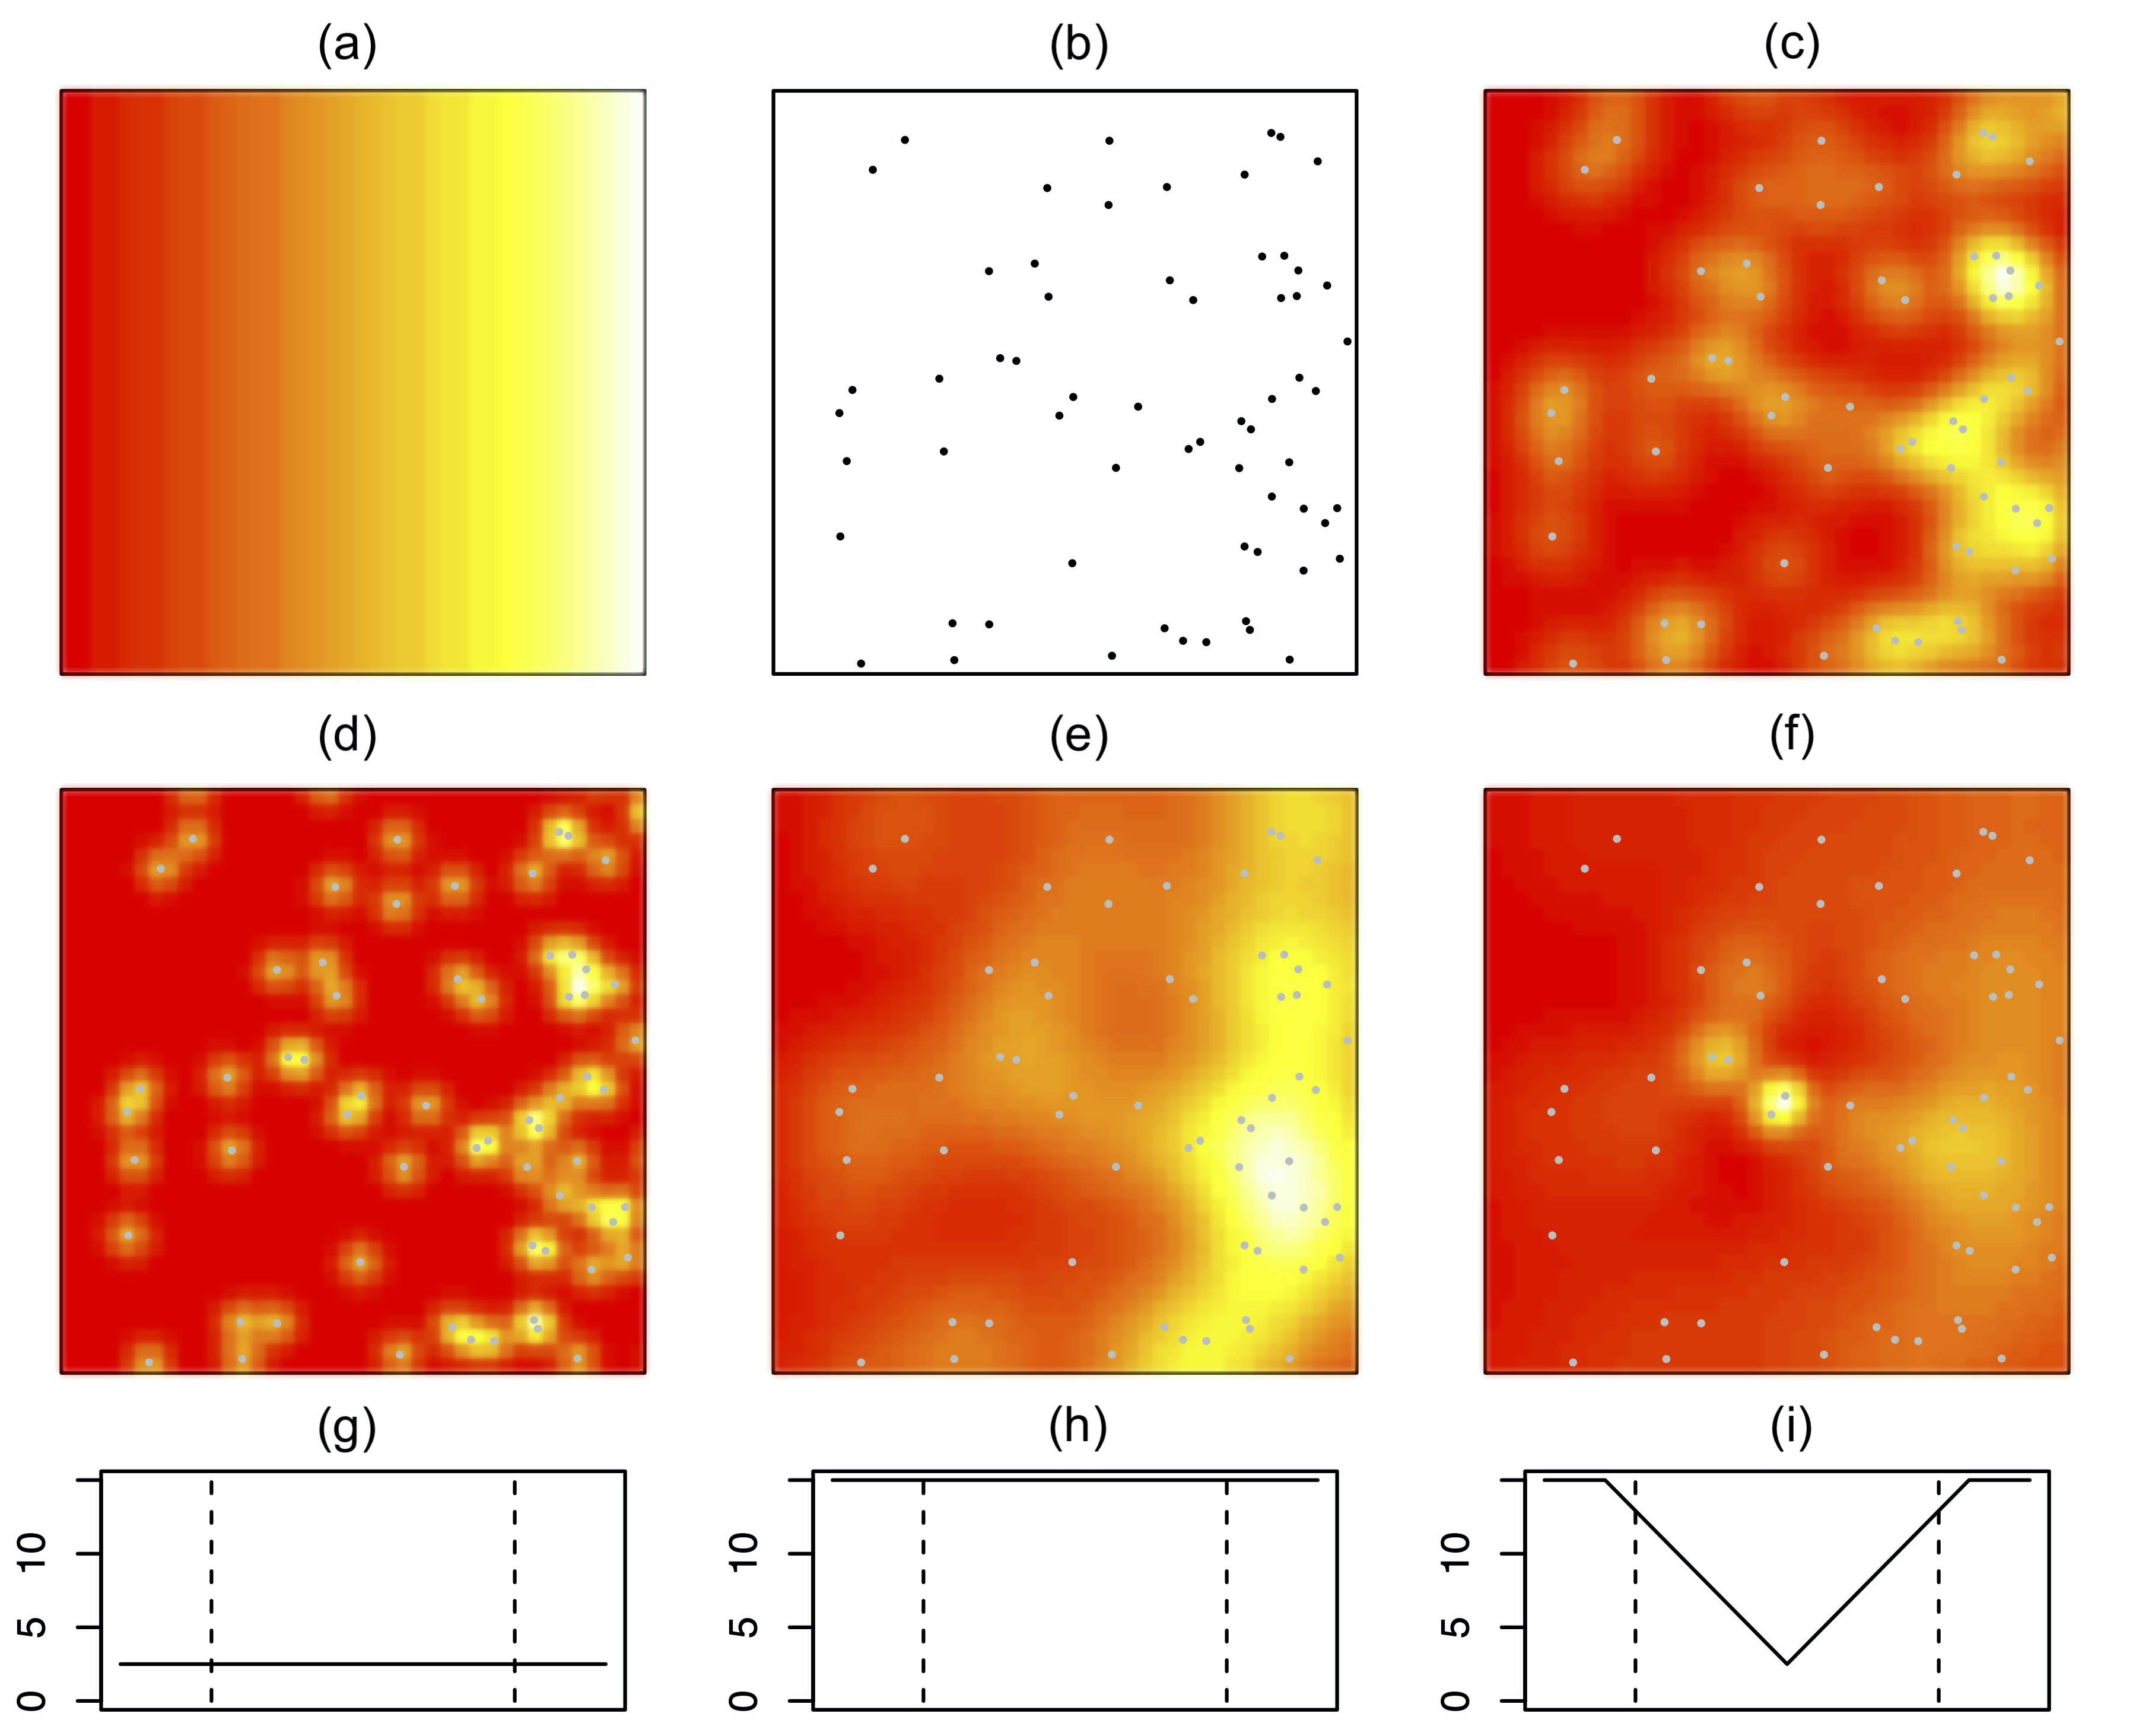
\includegraphics[width=\textwidth]{example-densities.jpg}
\caption{Examples of (a) an AC intensity (density) surface, (b) a realisation of ACs from this intensity surface. Panels (c) to (d) show the realised AC density in (b), when the individual AC PDFs ($f_1(\bm{s}),\ldots,f_N(\bm{s})$) are bivariate normal with standard errors (c) $\sigma=2.5$, (d) $\sigma=15$, and (e) $\sigma=2.5$ for an AC at the centre of the plot (dimension 100$\times100$), rising linearly to $\sigma=15$ by the edge of the plot. True ACs shown as grey dots. The colour scales of panels (c) to (e) are such that the highest and lowest densities in each plot is the same. Panels (f) to (h) plot the standard errors of the AC PDFs in (c) to (e) against the x-axis. Vertical dashed lines show the extent of the survey region in panels (c) to (e); a buffer beyond this is included because points outside it affect the plot within the survey region. Color version of figures can be found in the electronic version of this article.}
\label{fig:densities}
\end{figure}

\subsection{Estimated density surfaces}

Figure~\ref{fig:densities} shows examples of both types of density, together with realised AC locations. If we are interested in explaining why density tends to be high in some places and lower in others, or in characterising the process that governs the distribution of ACs, then we are primarily interested in estimating a density surface like that shown in Figure~\ref{fig:densities}(a). In this example, it is easting that influences this density, but in general it might be any of a wide variety of habitat or environmental covariates, some of which may be unobserved and evidenced only by spatial clustering of ACs. 

If we are interested only in where the ACs are, and not in explaining why they are there, then Figure~\ref{fig:densities}(b) suffices. With SCR methods we typically cannot observe ACs, but we can model the PDFs of ACs, and construct a density surface using Equation \eqref{eq:realised-D}. For example, Figure~\ref{fig:densities}(c)-(e) shows PDFs of AC locations when the individual AC PDFs are bivariate normal distributions with small variance in (c), larger variance in (d), and variance increasing linearly from the centre of the plot in (e). The PDFs ``spread'' information about each AC's location according to a bivariate normal distribution, with greater spreading when there is greater uncertainty about location (greater variance).

Ignoring the actual AC dots (because they cannot be observed), Figure~\ref{fig:densities}(c) gives a reasonable visual representation of where the ACs are. It is much more difficult to pick out individual ACs from Figure~\ref{fig:densities}(d), but it gives a reasonable representation of where the high- and low-density regions of ACs are -- much like Figure~\ref{fig:densities}(a), but customised somewhat for this particular realisation of AC locations rather than their long-run average locations. Note, however, that these two figures are representations of exactly the same set of ACs and that if one interprets them as plots of AC density, they contradict each other. Figure~\ref{fig:densities}(c) says that almost all the region has low density (red in the plot) and that there are lots of small high-density regions, while Figure~\ref{fig:densities}(d) says that there is much less variation in density, that there are large swathes of higher density (the yellow towards the right) and large swathes of low density towards the left. The reason that Figure~\ref{fig:densities}(d) shows less variation in density is not that there is less variation in the population (there are exactly the same ACs in both (c) and (d)), it is that we are less sure about the location of the ACs in (d). To interpret this as less variation in AC density is to invite incorrect ecological inferences.

Now what about Figure~\ref{fig:densities}(e)? If this is interpreted as indicating where the high and low-density regions are, it is misleading. It says that the highest density region is in the centre of the plot, and that the region with most variation in density is the central region, which is not true. 

The fact that there is only small uncertainty about AC location in the centre of the plot and large uncertainty error at the edges means that the ACs near the centre are not ``spread'' much and therefore appear as higher peaks in the surface, with low regions where there are no ACs. Near the edges of the plot, on the other hand, uncertainty about AC location is high and ACs are ``spread'' a lot, which both flattens the peaks at individual AC locations and ``fills in'' the troughs where there are no ACs. 

It is a feature of SCR surveys that the AC locations of individuals farther from the detector array tend to be estimated with greater uncertainty than individuals within the array. This is illustrated in Figure~\ref{fig:screrr}, which shows the estimated probability density functions for ACs of two animals detected on a simulated SCR survey with a 4$\times$4 array placed in the centre of the population shown in Figure~\ref{fig:densities}(b). The reason contours in the top right of the figure ``avoid'' the triangle is because the detection function range, estimated from the whole survey, not just the points shown, is large and if the AC was near the triangle, other detectors would have high probability of detecting it. The fact that they did not makes them ``repel'' the AC. 

\begin{figure}[htbp]
\centering
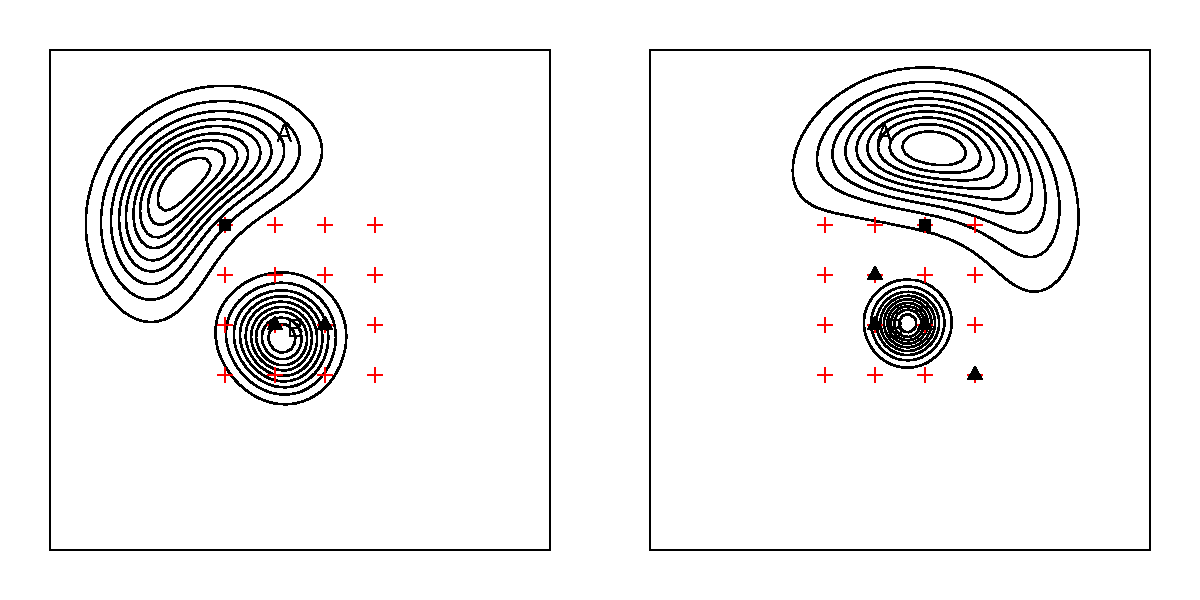
\includegraphics[width=0.5\textwidth]{screrr.pdf}
\caption{Estimated probability density function contours for two detections in an SCR survey of the population shown in Figure~\ref{fig:densities}(b). Detectors are shown as red crosses. The lower left individual was detected at detectors indicated by black squares, the upper right individual only by the top right detector indicated by a black triangle.}
\label{fig:screrr}
\end{figure}

\section{SCR density estimation methods} \label{secrmethods}

Maximum likelihood (ML) and Bayesian SCR estimation methods are documented in a good number of papers, starting with \cite{Borchers+Efford:08} and \cite{Royle+Young:08}. Both ML and Bayesian inference are based on SCR likelihood functions that include a component specifying the AC density surface, which may depend on spatially-referenced covariates (the linear density surface shown in Figure~\ref{fig:densities}(a) is an example), as described in Section \ref{different-densities}. ML and Bayesian methods are able to estimate $\beta_0,\ldots,\beta_K$, and hence estimate the expected AC density surface. 

Given spatial capture histories, ML and Bayesian methods are also able to estimate the locations of ACs (like those shown in Figure~\ref{fig:densities}(b), for example). While ACs are points, there is always uncertainty associated with estimating their locations, so that SCR estimates of AC locations are probability density functions (PDFs), not points. Estimates of these PDFs are conditional on the spatial capture histories of the individuals concerned -- because the capture histories contain the information on where each animal's AC was (see the capture histories and estimated location densities in Figure~\ref{fig:screrr}, for example). We denote the PDF for the location of the $i$th individual, with capture history $\bm{\omega}_i$, as $f_i(\bm{s})$. Details of how one obtains these estimated AC PDFs are contained in Section 4.3 of \cite{Borchers+Efford:08} for ML methods and the section ``Estimating derived parameters'' on page 3238 of \cite{Royle+al:09b} for Bayesian methods.

Note that we can obtain AC PDFs for undetected animals, because although the animals were unobserved, we know their capture histories -- namely no capture at every detector. We denote the PDF for these undetected individuals as $f_u(\bm{s})$. Note also that all undetected animals will have the same AC PDF because they all have the same capture history (unless there are individual-level covariates that affect detection probability estimates, a complication that we ignore here). 

Suppose that we estimate from an SCR survey that there are $\hat{N}$ animals within the survey region, $\mathcal{S}$. If one adds up the AC PDFs for all $n$ detected and $\hat{N}-n$ undetected animals, at all points in the survey region, one gets an estimate of the surface $D_r(\bm{s})$ of Equation~\eqref{eq:realised-D},
\begin{equation}
\widehat{D}_r(\bm{s}) = \sum_{i = 1}^n \hat{f}_i(\bm{s}) + (\widehat{N} - n)\hat{f}_u(\bm{s})
\end{equation}
with $f_i(\bm{s})$, $f_u(\bm{s})$ and $N$ estimated by SCR. This function is usually plotted after discretising the survey region into cells, with the estimated density in cell $j$ being $\widehat{D}_{rj}=\int_{\mathcal{C}_j}\widehat{D}_r(\bm{s})\, d\bm{s}/a_j$. It is this surface that many publications (including those listed in the Introduction) interpret as a density surface for AC or animal locations. While perhaps done for brevity, referring to the realised AC density surface as an estimated density of {\it animals} makes the additional error of ignoring animal movement around ACs. An AC PDF captures only uncertainty about where the AC is located. It is not equivalent to an estimate of the animal's home range. 

%This is an estimate of the realised AC density. It has been referred to as the estimated distribution, or density of \textit{animals}. However, animals distribute themselves around their ACs, so that AC density and animal density are not the same thing. Suppose for example, that we are certain that there is exactly one AC in a region that has area 1 (so that AC density in this region is 1). Suppose also that the animal with an AC in this region ranges wider than this region, and spends exactly half its time in this region. It is not certain that there is an animal in the region at any time, so that animal density will be less than 1. In this example, it would be fair to say that the \textit{animal} or \textit{usage} density in the region is 0.5. In this paper we focus only on the estimated AC density surfaces described in Sections \ref{s:eacd} and \ref{s:racd}.

\section{Methods}

We illustrate what each estimated surface gives the practitioner, and which interpretations are valid and useful, by simulating data from a density surface that has an easy visual interpretation. To do this, we turned one of the most recognisable images in Western culture, the Mona Lisa, into a density surface. We created a greyscale version of a region of the original image (Figure \ref{mlinputs}a) in which values give the intensity of the point process generating ACs, and lighter areas correspond to higher densities. The intensity surface is continuous, with intensities defined at any point $\bm{s}$. Although any pixelated image must be discrete at some scale, the resolution we use in Figure \ref{mlinputs}(a) is sufficiently high (1200$\times$ 1200 pixels) to visually make the point that the surface is continuous.  

The image's pixel intensities can be arbitrarily scaled to integrate to the expected number of activity centres over the surface. We chose this to be 80, on the basis that this is sufficient to illustrate our main points and also broadly typical of many wildlife surveys. We then generated a single realisation of points from this surface (from an inhomogeneous Poisson process with average intensity of 80), which resulted in 85 ACs being generated (Figure \ref{mlinputs}(b)).

\begin{figure}[htbp]
\centering
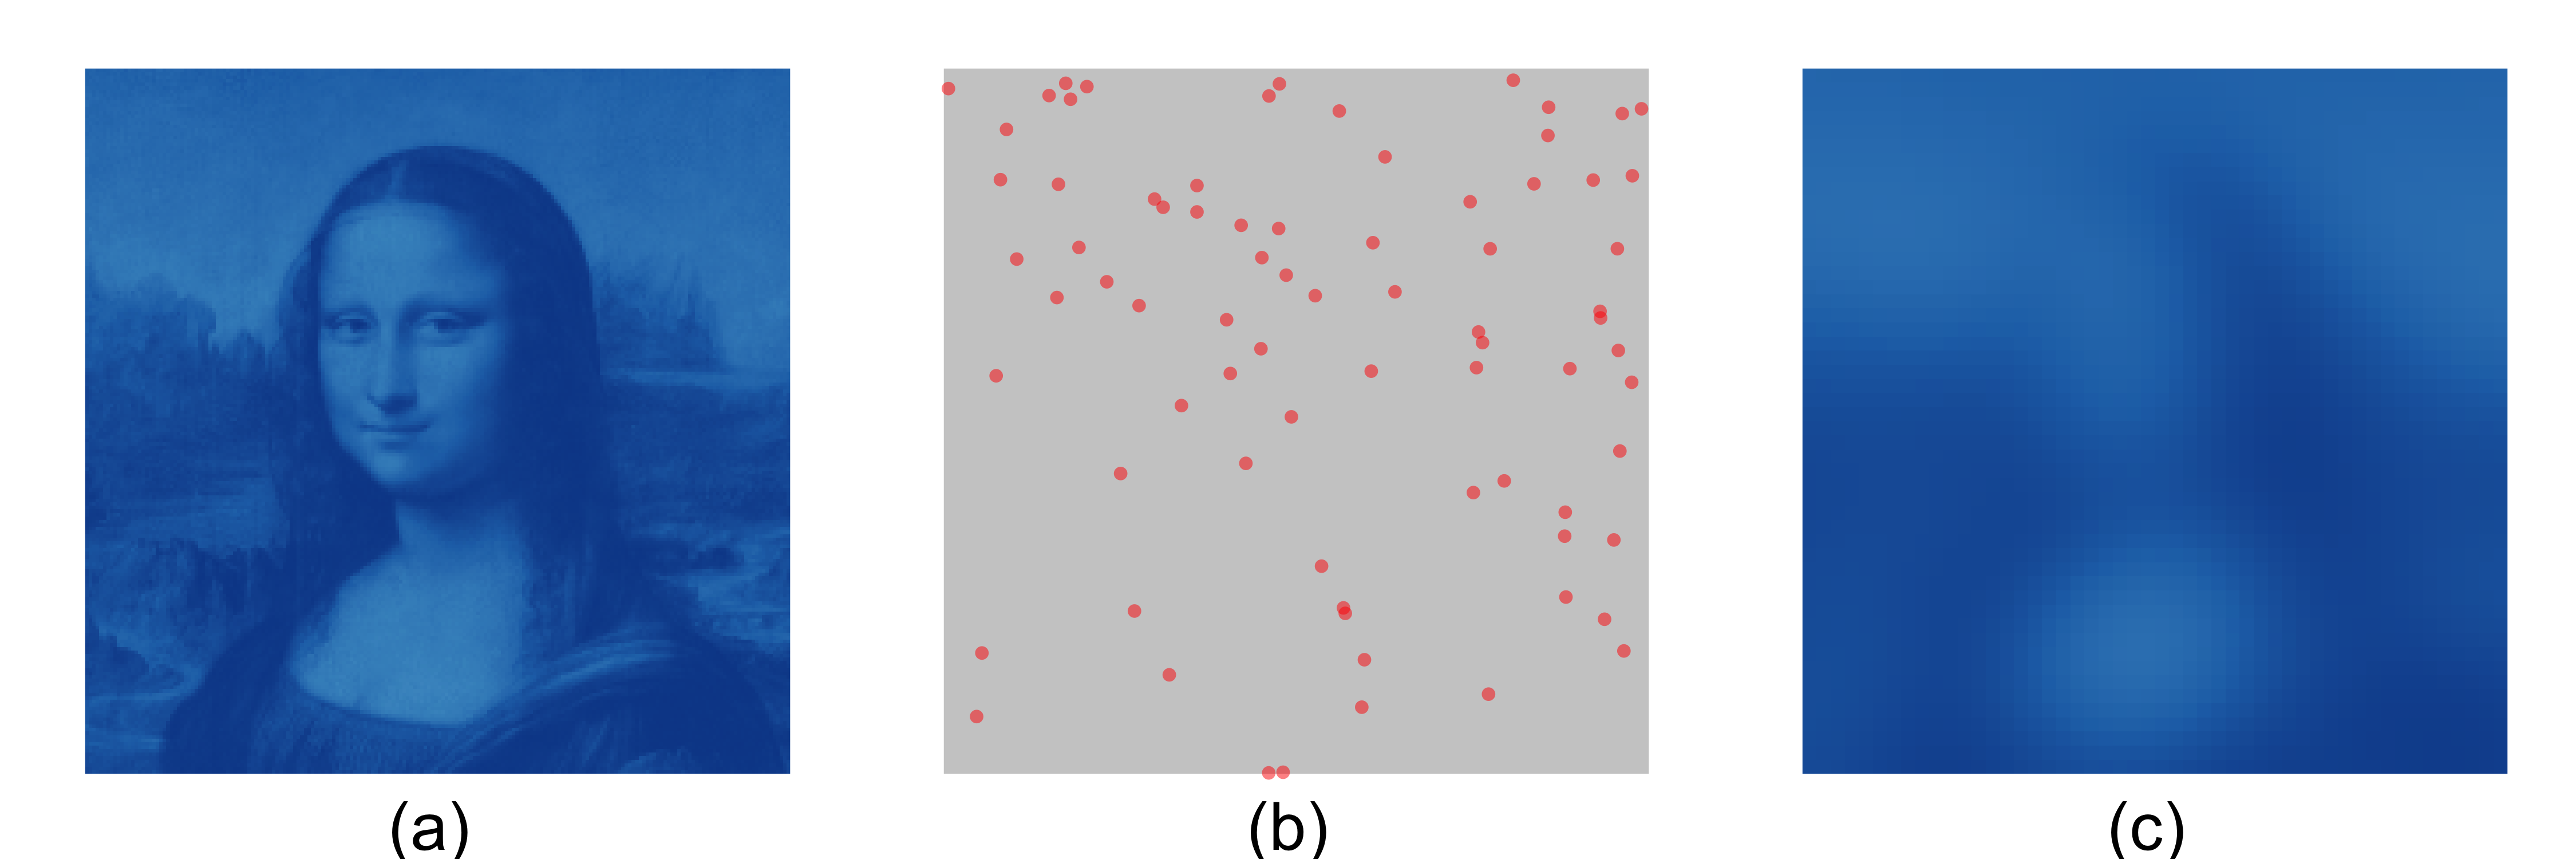
\includegraphics[width=1\textwidth]{mona_inputdata.png}
\caption{Input data for the Mona Lisa simulation study. Panel (a) shows a greyscale version of the Mona Lisa treated as an expected AC density surface. Panel (b) shows a single realisation of 85 ACs generated from the surface in (a), while (c) shows a spatially-varying covariate that is correlated with true density, and which is used to estimate expected AC density surfaces.}
\label{mlinputs}
\end{figure}

We simulated capture histories from the population using a half-normal encounter rate function $\lambda(d) = \lambda_0\exp\{-d^2/(2\sigma^2)\}$, where $\sigma$ is a scale parameter determining how quickly the encounter rate decreases with $d$, the distance between the detector and the activity centre, and $\lambda_0$ is the expected number of encounters at a detector that is at animal's AC ($d=0$). Arbitrarily defining the dimensions of the image to be $50\times 50$ units, we set $\sigma=4$ and used two different detector arrays: a $3\times3$ array centred at $x=18$ and $y=24$ (Figure~\ref{mona3x3}), and a $7\times 7$ array covering the entire image (Figure~\ref{mona7x7}). Note that the survey region is closed, in the sense that there are no detectable ACs beyond its borders. Both arrays had a fixed spacing of $2\sigma=8$ between detectors. The number of simulated detections at each detector were Poisson random variables with expected values equal to the encounter rate function evaluated at the distances of detectors from ACs. In order to illustrate how realised and expected AC density surfaces change with increasing sample sizes, we simulated capture histories with three different survey effort levels, obtained by varying $\lambda_0$ so that the average number of detections per detected individual was approximately two, four, or eight (corresponding to $\lambda_0=1.8, 5.2$, and $11.1$ for the $3\times 3$ grid, and $\lambda_0=0.7, 2.5$, and $5.5$ for the $7\times 7$ grid). This generated between 47 and 318 detections of between 23 and 39 individuals for the $3\times 3$ grid (Figure~\ref{mona3x3}), and between 94 and 702 detections of between 54 and 85 individuals for the $7\times 7$ grid (Figure~\ref{mona7x7}).

Parameter estimation by ML SCR methods requires numerical integration of the likelihood, which is facilitated by defining a fine mesh of points at which the likelihood can be evaluated. This mesh, sometimes called the habitat mask, has the effect of discretizing continuous space into grid cells, with the mask points at the centres of the cells. We used a $50\times 50$ habitat mask i.e.\, a spacing of $1=\sigma/4$ between mask points. To estimate the realised AC surface, we assumed a model with constant density. 

To estimate an expected AC density surface, we generated a covariate by blurring the true density surface at the resolution of the habitat mask (Figure~\ref{mlinputs}(c)). Pixel intensities were rescaled after blurring so that the number of expected activity centres remained the same as in the original surface (i.e., 80). Because it is based on true density, the covariate is very informative about the true densities, although the strength of the association is diluted by the blurring. We estimated an expected AC density surface assuming a model in which density is a function of covariate values. Note that, because density is parameterised with a log link (see Section \ref{secrmethods}) but the blurred surface is obtained directly from the true density surface (so that $D(\mathbf{s})\approx x_1(\mathbf{s})$, with the degree of blurring determining the accuracy of approximation), covariate values were log-transformed to ensure the model was correctly specified.%\todo[inline]{dlb: this seems a bit more convoluted than necessary - why not just plot the logged covariate and leave it at that?}

Most of the examples of unclear or incorrect interepreations of density surfaces that we listed in the introduction are made using Bayesian methods. To show that correct interpretations do not depend on the inferential method used, models were fitted by both ML, using the \texttt{secr} (v4.5.4) package\footnote{Realised AC density surfaces can be produced in \texttt{secr} with function \texttt{fx.total}. Documentation warns the user that ``the surface represents what is known from the data about a specific realisation of the spatial point process for home range centres: varying the intensity of sampling will change its shape. It is not an unbiased estimate of a biologically meaningful density surface.''} \citep{secr:21} and Bayesian inference, using custom code written using the \texttt{NIMBLE} package \citep{deValpine:17, Turek:21} in R version 4.1.2. We report the ML estimates here; the Bayesian estimates are not materially different and are reported in Supplementary Material A.

\subsection{Results}
The most striking features of the realised AC density surface estimates shown in Figure~\ref{mona3x3} (top row) are that (a) they do not really recover the Mona Lisa in any recognisable way, (b) they predict flat density far from the array, (c) they become more ``spiked'' (density concentrated more closely around estimated AC locations) inside the array as sample size increases, and (d) the distance from the array at which the surface becomes flat increases as sample size increases. We discuss each of these features below

Regarding (a), realised AC surfaces are not designed to recover the expected density of ACs (which is what the Mona Lisa image is). They are designed to provide information about the locations of ACs in the surveyed animal population, given the data observed. Point (b) is a consequence of this: because ACs far from the array are not detected, there is no information in the sample on their location other than that contained in the SCR estimate of mean density, and so all the model ``knows'' about ACs far from the array is that they occur in space at the estimated mean density of ACs. Point (c) and (d) are further consequences and essentially reflect the same phenomenon: as sample size increases, more information is collected on where ACs in the vicinity of the detectors are, and so the probability density of each estimated AC location contracts. Increasing survey effort increases sample size in two ways: animals already detected can be detected again, and animals not yet detected can be detected for the first time. Point (c) occurs because animals with ACs in the interior of the array tend to be detected most often. Point (d) occurs because increasing survey effort results in first detections of peripheral animals further away from the array, replacing their previous flat contributions to the surface with contributions that have some relief. This has the visual effect of pushing back the flat part of the surface and extending what is considered the periphery or ``in the vicinity'' of the array. 

Introducing covariates into the density model allowed us to recover features of the Mona Lisa across the entire image, not just near where detectors were located (Figure~\ref{mona3x3}, bottom row). Recovery may not be this good in reality -- we simulated our covariate to be strongly related to true density -- and extrapolation so far beyond the area where data was collected may be ill-advised in practice. Notwithstanding this, it is true in general that because the expected AC surface depends on the relationship between the covariate and density, the model uses estimates of this relationship obtained where it has lots of information (within the array) to infer density beyond the array. The inferred surface is also relatively insensitive to sample size.

The realised AC density surface estimates in Figure~\ref{mona3x3} are misleading if interpreted as AC density plots, not because uncertainty about AC locations depends on sampling intensity, but because there are systematic spatial differences in this uncertainty (uncertainty is greater on the periphery of the array than inside it), and so spatial differences in AC density are confounded with spatial differences in uncertainty. Spatial differences in uncertainty are minimized if the survey region is closed and surveyed with even intensity (Figure~\ref{mona7x7}, top row). Realised AC density surface estimates then provide a fair indication of AC distribution, although uncertainty will still be greater near the boundary of the survey region (because fewer detectors are within reach of an AC near the boundary than an AC that is well within the array). 

Where the survey region is not closed but has been evenly surveyed with a large, regular array, a similar effect can be achieved by restricting inference to the interior of the array, except that animals with ACs in the periphery outside the array will still make a contribution to the restricted surface. Note that, in contrast to the realised surfaces, the expected AC density estimates in Figure~\ref{mona7x7} (bottom row) are very similar to those in Figure~\ref{mona3x3}. 

\begin{figure}[htbp]
\centering
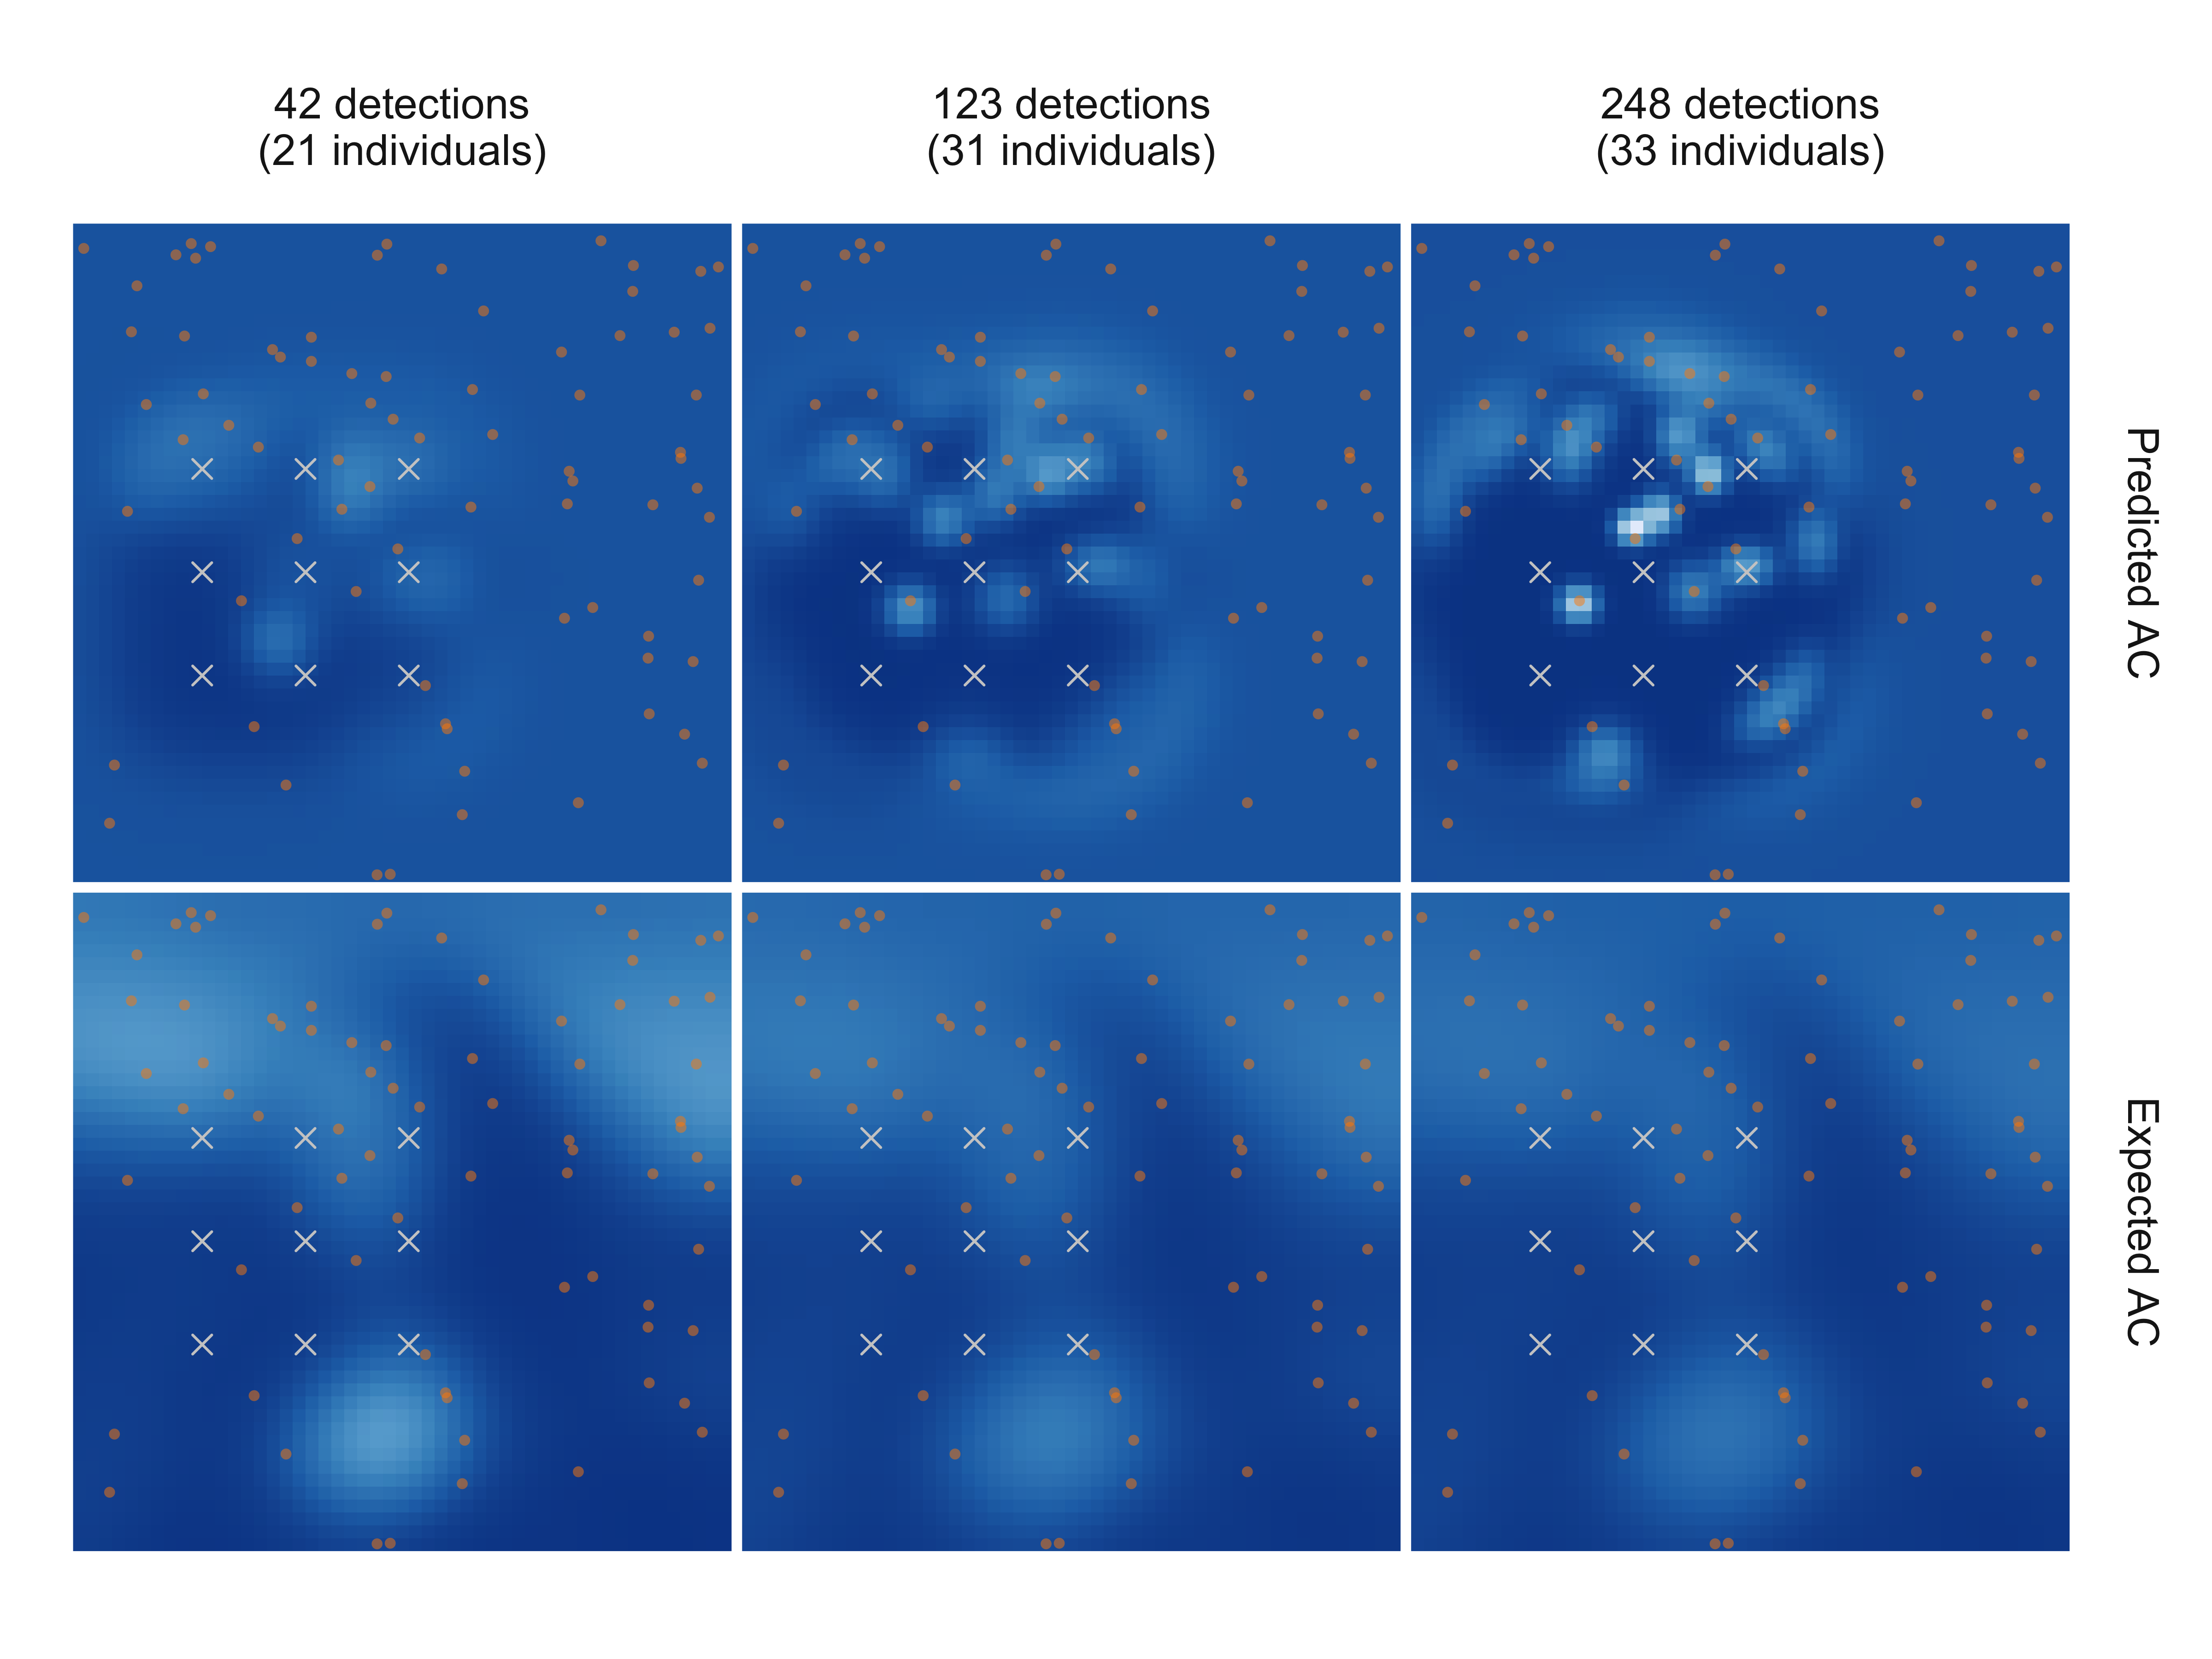
\includegraphics[width=1\textwidth]{mona_3x3.png}
\caption{Plots (a), (b), (c) show estimated realised AC surfaces estimated using the 3$\times$3 array indicated by grey crosses under three levels of survey effort. True AC locations are shown as orange dots. Plots (d), (e), (f) show expected activity centre surfaces estimated using a model in which density is a function of a simulated spatially-varying covariate (see Figure \ref{mlinputs}c).}
\label{mona3x3}
\end{figure}


\begin{figure}[htbp]
\centering
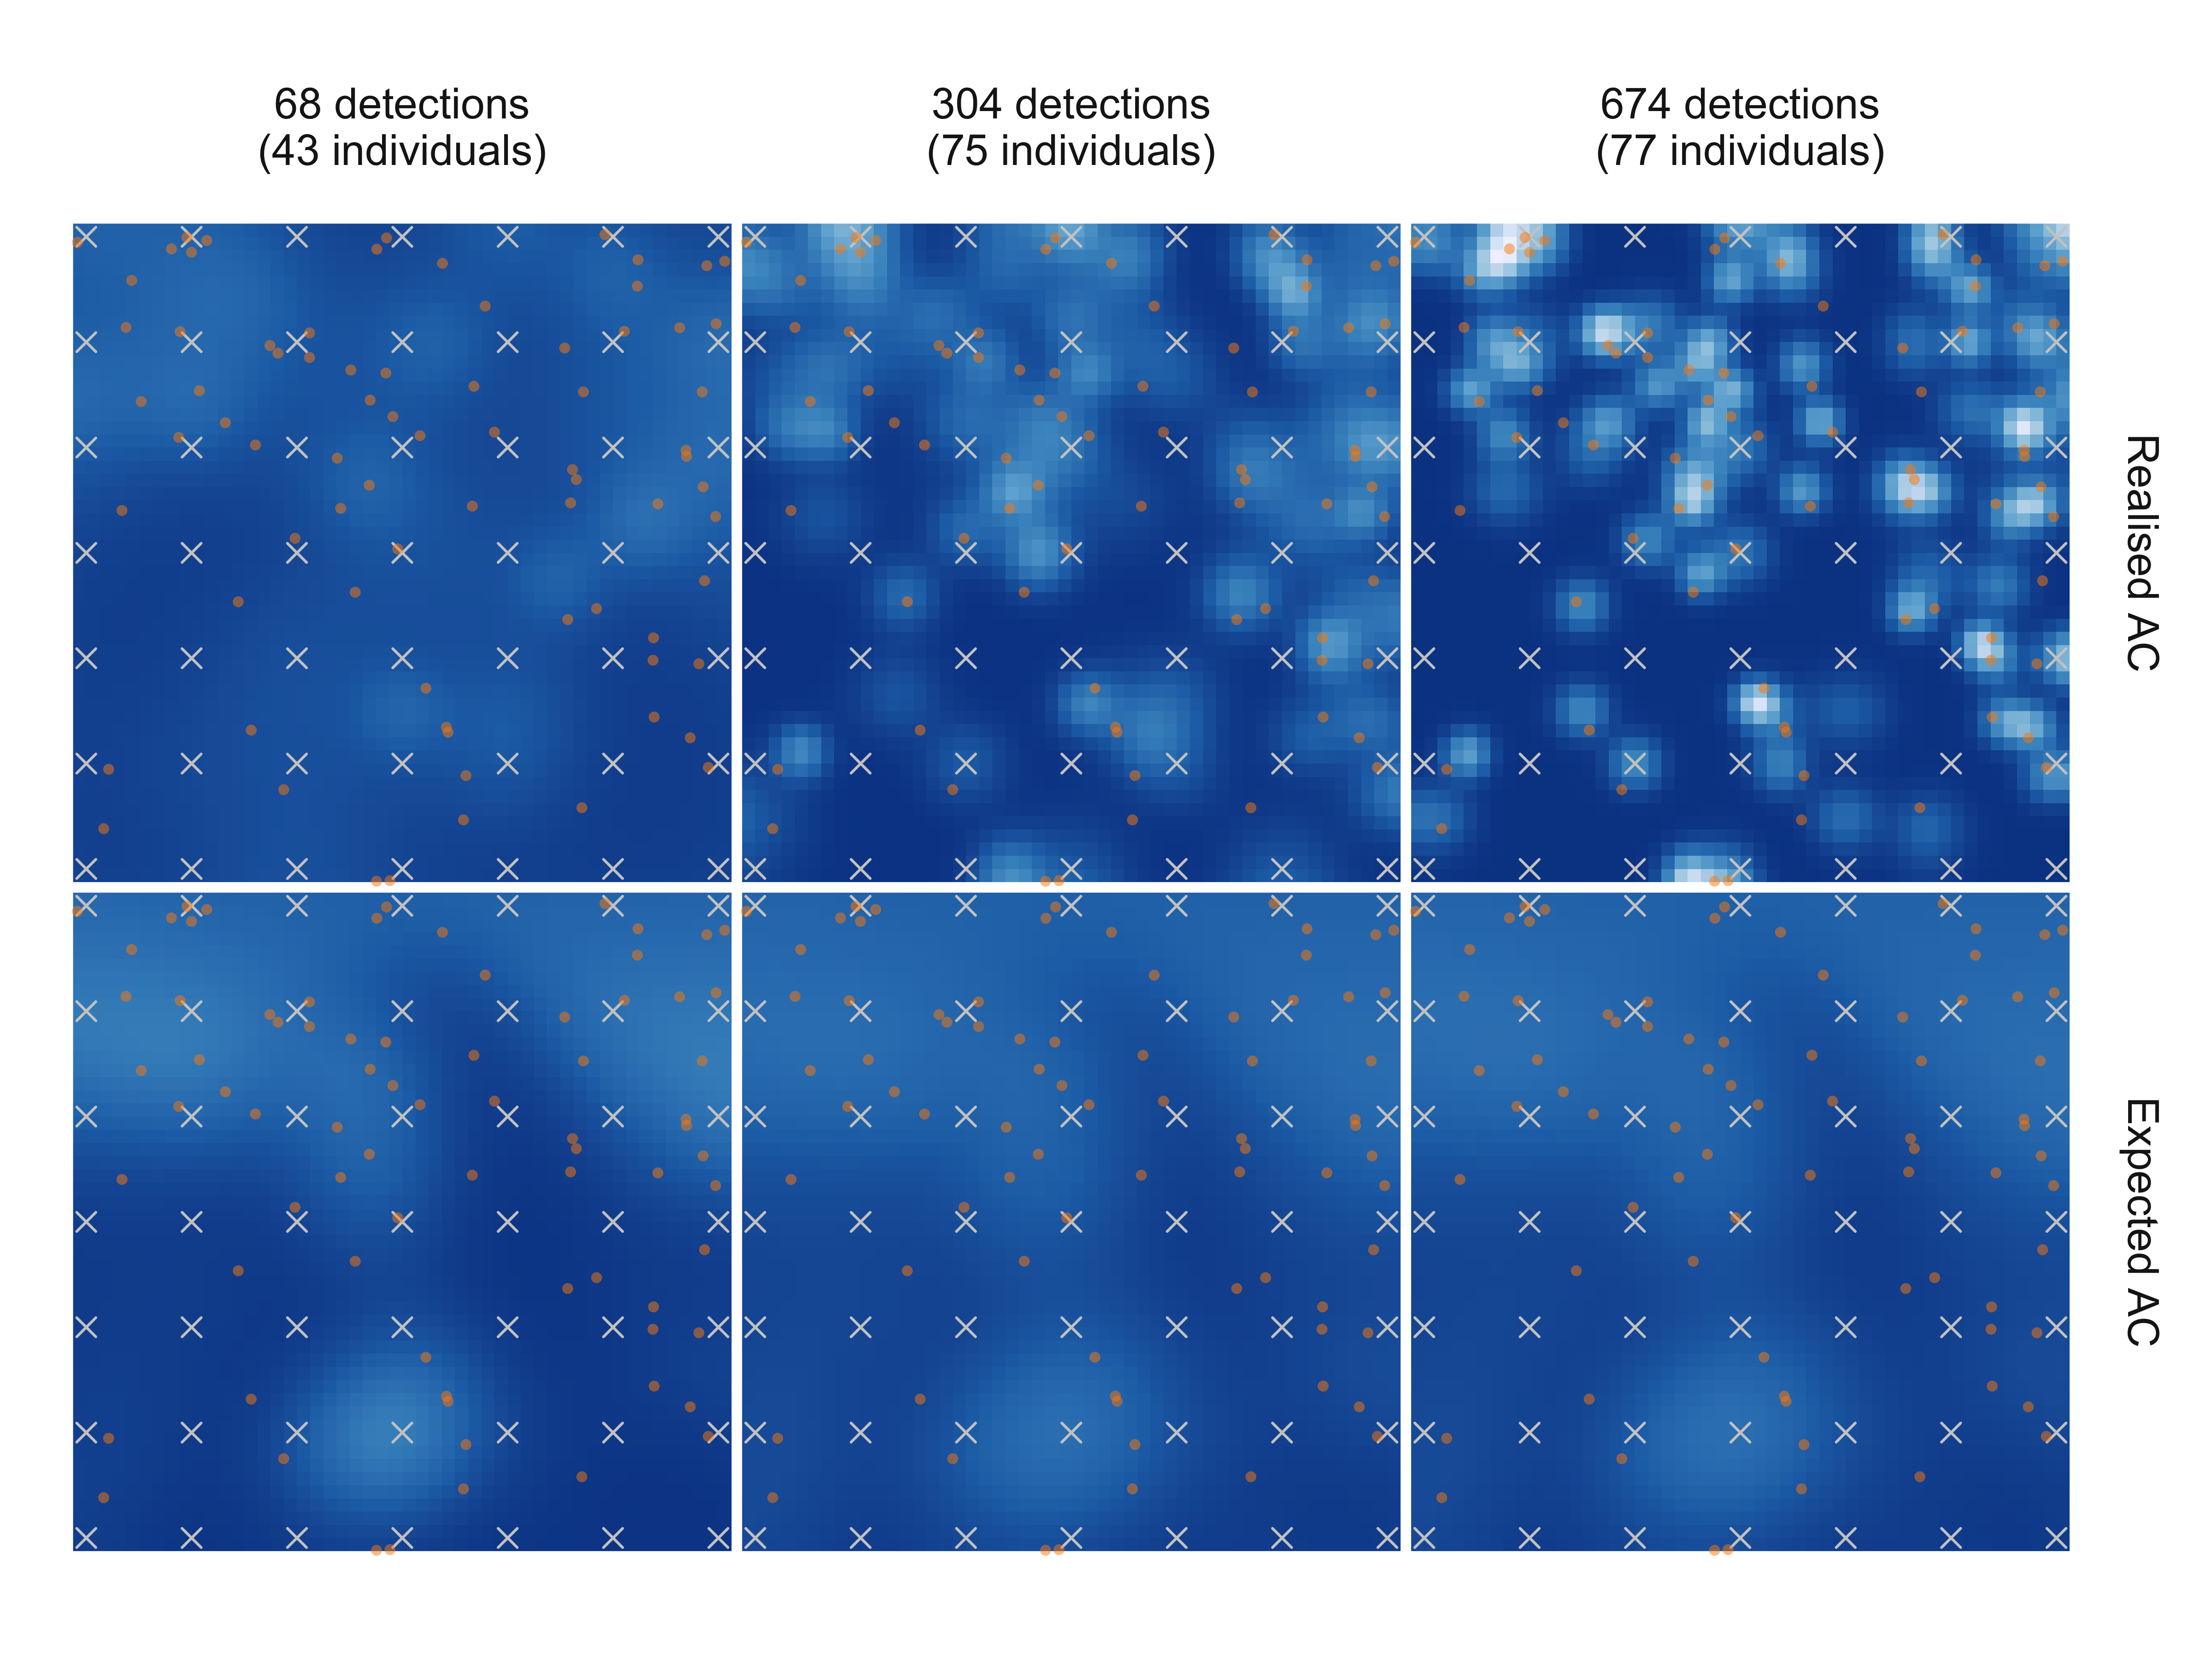
\includegraphics[width=1\textwidth]{mona_7x7.png}
\caption{Plots (a), (b), (c) show estimated realised AC surfaces estimated using the 7$\times$7 array indicated by grey crosses under three levels of survey effort. True AC locations are shown as orange dots. Plots (d), (e), (f) show expected activity centre surfaces estimated using a model in which density is a function of a simulated spatially-varying covariate (see Figure \ref{mlinputs}c).}
\label{mona7x7}
\end{figure}

\section{Discussion and Conclusions} \label{discussion}
%\todo[inline]{dlb: Seemed to me that we could usefully combine discussion and conclusions, so I have done that.}
%\todo[inline]{ Key points (maybe one per para?): (1) RACD misleading because spatial diffs in AC density are confounded with spatial diffs in uncertainty [[Do we need to disentangle here (a) that increases in survey effort make the surface more peaked (which is a problem if interpreting purely as AC density but not if you keep uncertainty in mind), (b) that there are systematic spatial differences in uncertainty (uncertainty increases as one moves away from the array), which is a bigger problem because you can't see how uncertainty is changing (because of the confounding). (2) Expected (long run good areas) vs Realised (where animals are in this population). (3) RACD is ok if even sampling across a closed region (even then not perfect, cos uncertainty still higher near the borders, but probably practically ok). (4) Covariate models provide EACDs, but obv depend on covariate. (5) Difficulty of showing uncertainty associated with densities (Ben/Rishika?). 
 
%Maybe start with ``Realised AC densities produced from an SCR model are in many instances misleading, because spatial differences in the density of AC locations are confounded with spatial differences in the uncertainty about these locations.'' }

%\todo[inline]{BCS: Is the following paragraph too strongly worded? We just said ``... Realised AC density surface estimates then provide a fair indication of AC distribution'' in the previous section. Maybe we could start this paragraph with ``In many cases, realised AC density surfaces...''}
For most practical surveys, the realised AC density surfaces produced from an SCR model cannot be interpreted as density maps in any meaningful biological or ecological way, because they depend heavily on factors related to the detection process that have nothing to do with the underlying AC density. 

The surfaces will always show less spatial variability far from the detector array than close to, or within it, whether the underlying density is less variable there or not. This point is clearly stated in \cite{Royle+al:13a}, who say (pp.\ 165--166) ``As we move away from `where the data live' (away from the detector array) we see that the density approaches the mean density. This is a property of the estimator as long as the detection function decreases sufficiently rapidly as a function of distance. ... predictions tend toward the global mean as the influence of data diminishes''. In addition, a survey that uses greater survey effort will produce a realised AC density surface that has more spatial variability than a survey of exactly the same animals using lower effort. And the spatial variability moves with the array: move the array and the regions of high and low realised AC density move with it, even though the true ACs do not move.

A useful metaphor here might be of SCR as a torch shining a light onto the true activity centres -- what you see depends on where you shine the torch (detector locations) and how brightly you shine it (survey effort). If you interpret the uniform darkness outside of the beam to mean that everything outside the beam is the same, you fundamentally misunderstand the nature of torches and will draw fundamentally incorrect conclusions.

%More importantly for people actually conducting SCR surveys is that the realised density estimates obtained in the periphery of the detector array, and even inside it, {\it also} depend on where detectors are located. 

When considering realised ACs, SCR models answer the question ``where is an animal with {\it this} spatial capture history likely to have its activity centre?'' The answer is always contingent on where detectors are located - because the capture history depends on where the detectors are located. This is the case regardless of whether one works in a Bayesian or frequentist framework. The same is true of the realised AC density surface, which simply sums estimated AC PDFs across animals, and will also be true for any downstream analyses that make use of realised AC densities e.g.\ density-weighted connectivity \citep{Morin2017}.

Uncertainty about the location of an animal's AC is affected by the number of times it is detected and the number of detectors it is detected at (and to some extent by the spatial configuration of those detectors). These quantities tend to be larger, and so uncertainty less, for animals whose ACs are within reach of more detectors. For a regularly spaced grid of detectors, this means that uncertainty is less for animals whose ACs are well inside the array than it is for animals whose ACs are near the border of the array. For irregularly spaced arrays (i.e.\ most surveys) systematic spatial differences in locational uncertainty exist within the array because sampling intensity is not uniform throughout the survey region -- detectors are by definition more densely clustered in some subregions than others. Concerns about spatial differences in uncertainty are diminished when the surveyed area is large and surveyed with even intensity, and under these conditions the realised AC density surface provides a reasonable reflection of the spatial distribution of ACs, particuarly within the array. But these conditions are not likely to hold in most SCR studies with typical resources.

To extend the metaphor, a torch beam's does not abruptly change from bright to dark. At the periphery of the beam (near the extent of the array) objects become increasingly difficult to see. Increasing the brightness of the torch makes everything within the beam easier to see, but also pushes back the periphery of the beam. And even in the interior of the beam, a bug on the glass (uneven sampling within the array) casts a shadow. Drawing a line at which the torch can no longer be trusted is to some extent arbitrary. 

\textcolor{red}{Communicating uncertainty in estimated density surfaces is one important issue we have neglected to mention so far for brevity. We recommend including plots of expected density surface estimates with plots that communicate standard measures of estimate uncertainty. For a frequentist analysis options include pixel-specific standard errors, coefficients of variation, and upper- and lower-limits of confidence intervals. Alternatives for a Baysian analysis include posterior standard deviations and credible interval limits. In Supplementary Materials A, we include upper- and lower-limits of credible intervals alongside the expected density surface estimates from our Bayesian analysis.}

\textcolor{red}{A confidence interval aims to capture a parameter for some nominal proportion of data realisations generated by the model. It does not make sense to construct confidence intervals for realised density surface estimates, because these surfaces aim to describe features specific to one single data realisation, rather than parameters that control the generation of all possible realisations. An interval constructed to describe uncertainty in a pixel's realised density estimate would reflect uncertainty in where activity centres are for this particular realisation, rather than uncertainty in estimates of the intensity surface that generated the activity centres. We are not aware of any publications that plot uncertainty in realised density surface estimates\todo{\textcolor{black}{Is this true?}}, but we highlight that any interpretations of this type of uncertainty should made with care, and that they are fundamentally different to interpretations of uncertainty in expected density surface estimates.}


% UNCERTAINTY STUFF: One way to see that flatness away from detectors reflects uncertainty rather than homogenous density is to plot lower and upper percentiles at each pixel, rather than just the posterior mean -- the differences between these percentiles would be large away from detectors and small close to detectors. It seems that this is rarely done, or at least reported in the literature; a practice that would be worth changing. 

%More importantly for people actually conducting SCR surveys is that the realised density estimates obtained close to detectors (and even inside the detector array) {\it also} depend on where detectors are located. The inset plots of Figure \ref{mona1low} and \ref{mona1hi} show the same region in space, and this region lies within a $2.5\sigma$ range of all detector arrays, where one would expect to be making inferences about activity centres. We obtained very different density surfaces in this area depending on where detectors were located. 

%When considering realised ACs, SCR models answer the question ``where is an animal with {\it this} spatial capture history likely to have its activity centre?'' The answer is always contingent on where detectors are located - because the capture history depends on where the detectors are located. %Changing the locations of detectors also changes the expected capture history, and thus the answer to the question of where the activity centre is located. 
%This is the case regardless of whether one works in a Bayesian or frequentist framework. The same is true of the realised AC density surface, which simply sums estimated activity centres across animals. In this case the question being addressed is ``Where are the animals with {\it these spatial capture histories} likely to have {\it their} activity centres?'' The dependency on detector location applies to activity centres estimated for detected animals and for those that were not detected. In the latter case we have limited information and the answer to the question for them is really just ``nowhere near where detectors are located''. 

%None of this precludes realised AC density surfaces from being useful sources of information, but they do need to be interpreted with care. Realised AC densities do not give proper answers to questions like ``where are the high- and low-density regions?'' because the highest and lowest points of the surface will always be at or near detectors; not because these are high- or low-density regions of space, but because this is where the capture histories make us most certain that animals are, or are not, present. They also cannot answer questions like ``are animals clustered in space?'' or ``is animal density heterogeneous?'' because the realised density surface will always exhibit variability, even if animal densities are truly a realisation of a homogeneous Poisson point process (and how much variability depends on how much survey effort was used).

%When estimating the location of a given activity centre, the bias caused by detector locations is lowest if the activity centre occurs near the centre of a dense array of detectors, and is highest if detectors are all on one side of the activity centre or if detections are only made at a single detector. Thus bias can be reduced by using a design that makes it likely that all activity centres in the study region are surrounded by a network of detectors. This will be unachievable for most wildlife surveys, as it requires a large number of detectors covering an area beyond the study region, and ideally placed at random {\it [[[note: I say `beyond the region' so that activity centres at the borders are also in the centre of some array, but not sure this is correct -- ????]]]} . In summary, it is incorrect to interpret the realised activity centre density surface as if it indicated where animals currently have their activity centres. \todo[inline]{DLB: The paragraph above seems both redundant (we have already made the point about misinterpretation of activity density surfaces quite well I think), and unclear in that I don't know what ``bias'' is being referred to in it. I suggest we remove the paragraph.}

There is a way of using SCR so that parameter estimates can be interpreted in a biologically or ecologically meaningful way, and this is by modelling the intensity of the underlying process as a function of environmental covariates. Covariates allow one to see beyond the spatial extent of the array (see bottom rows of Figures~\ref{mona3x3} and \ref{mona7x7}), provided that the relationship between covariate and response is a good one, and that detectors cover a sufficient range of covariate values to estimate that relationship well. The resulting surfaces show the (estimated) intensity of the underlying process assumed to generate activity centres. These expected densities will be highest where environmental covariates are most favourable. Using covariate models, and associated model-based inference, is not without issues -- there is a danger of extrapolating the density surface beyond the range of covariates around the detectors, particularly with a log link function, and the relationship with density and covariate is assumed to be the same everywhere as it is around the detectors. Notwithstanding this, expected AC density surfaces are no longer strongly tied to one particular realisation of the Poisson process or to where detectors are placed.

%Rather, they answer the questions ``Where are the high- and low-density regions?'' and ``What spatial variables are good predictors of the high- and low-density regions?'' 
%in a way that is consistent with how this question is answered by species distribution models. %They predict where we would expect to see activity centres, if we were able to observe multiple independent populations distribute themselves across the study region. 

%Using covariate models, and associated model-based inference, is not without issues -- there is a danger of extrapolating the density surface beyond the range of covariates around the detectors, particularly when using a log link function, and the relationship with density and covariate is assumed to be the same everywhere as it is around the detectors. %The extent to which the expected activity centre surface predicts where animals have their activity centres {\it in this realization of the process} depends on the strength of the covariate relationship and on the number of activity centres, each of which is assumed to be an independent draw from the underlying process. %In the Nagarahole survey, for example, there is a relatively weak northing covariate and a relatively small number of activity centres, and the estimated expected activity centre density surface provides very little information about the location of current activity centres. 

%\todo[inline]{dlb: I have commented out all mention of usage surfaces. This is what we agreed, isn't it?}
%The concept of an activity centre is central to SCR models, but for many applications of SCR it may be more appropriate to consider a distribution of space use, taking into account all locations where an animal may have been present, rather than a distribution over activity centre locations only. The detection function or encounter function estimated as part of an SCR model provides information about how far from its activity centre an animal may move. This can be easily integrated with the estimated realised AC density to give an estimated realised {\it usage} density surface. The resulting surface effectively smooths the realised AC density surface, with the amount of smoothing determined by the distances that animals move. As it is based on realised AC density, the usage density surface also depends on where detectors are located and on survey effort. However, it depends less heavily on these factors than the realised AC surface because the detection function or encounter function does not depend on them. In particular, the realised usage density surface quickly stops becoming increasingly ``peaked'' as survey effort increases.

%We constructed individual usage distributions using the encounter function from our SCR model, but this may not always be appropriate. For example, if individuals cannot fully explore their home range within the duration of the survey, then we would not expect the spatial range of the detection function to match the extent of an animal's usage distribution. Even for longer surveys, it may not be sensible to relate the range of the encounter function to the size of the region used by an individual even for longer surveys, so care should be taken when this practice is used. For example, \cite{Tenan+al:17} found that the spatial scale of the encounter rate function for brown bears (\emph{Ursus arctos}) estimated using SCR was not consistent with spatial usage parameters estimated from other data sources, although \cite{Popescu+al:14} did not detect any such inconsistency for a population of fishers (\emph{Pekania pennanti}). If alternative data sources are available (e.g., telemetry, or opportunistic data such as hair or scat samples) they may be incoprorated for improved estimation of individual usage distributions \citep{Tenan+al:17}. Our method also assumes that home ranges are circular, however their shapes are likely to be modified by variables relating to population and landscape connectivity \citep[see][for a review]{Drake+al:ip}.

Ultimately, the appropriate density surface to use depends on the aims of the researcher. We have argued that the estimated realised AC density surface should not be used, because of the strong dependence on detector location and survey effort. But if the goal is to identify the ACs of {\it some} animals currently in the study region (and it does not matter which ones) then it may well be an efficient way of locating these, especially in the interior of large, evenly sampled survey regions. If the goal is to estimate where animals (not just the ones in the current realisation) are likely to have activity centres, then the expected AC surface, with density a function of covariates, should be used.

%\section{Conclusions}
%This paper demonstrates that the summed posterior distribution of estimated ranges across animals obtained from SCR -- what we call the realised activity centre density surface -- cannot be used as a species distribution model. We illustrated this point in a number of ways, first with a binomial point process, then by using the Mona Lisa to simulate a Poisson point process, and finally using data from a real-world camera detector survey. All these examples returned the consistent message that realised activity centre density surfaces differ depending on detector location. This dependency is most obvious at large spatial scales, where moving a detector array is like ``shining a torch'' on a particular part of the study area, but is also present within the region in and around the detector array itself. 

%Our main messages are:
%\begin{enumerate}
%\item Realised activity centre density surfaces cannot be interpreted as SDMs. This is both because these surfaces draw inferences about one realisation of a spatial point process, whereas SDMs make inferences about the long run average of the process; and because the surface depends systematically on where detectors are located.
%\item The realised activity centre density surface typically shows highest peaks and deepest troughs close to the centre of arrays, defaulting to close to the mean of the underlying process away from the array. A flat density away from detectors reflects a lack of knowledge, and not constant density. We should expect that in reality some areas away from detectors have substantial deviations from the process mean -- it is just that we do not know which areas.

%\item An SCR model that models mean activity centre density as a function of environmental covariates can be interpreted as a SDM. Here the key difference is that the surface obtained from the covariate model -- what we call an expected activity centre surface -- is a statement about the mean intensity of the underlying process, and is independent of array location provided that the environmental covariate space has been sufficiently sampled.

%\item Realised activity centre densities can be extended into realised usage densities. This is done by using the estimated encounter rate function to ``spread'' animals about their estimated ACs according to the expected number of encounters of the animal as distance from its AC increases. 
%\end{enumerate}

%"OK everyone, put your detectors where you'd like to shine your torch, and you'll get a perfectly good estimate of animal density there using our posterior AC map".

\section*{Acknowledgements}

This work was part-funded by the Royal Society of New Zealand through Marsden grant UOA-1929.

%\section*{Conflict of interest statement}
%
%The authors declare no potential conflicts of interest.

\section*{Data availability}

All data and code used in the paper, along with model objects and results, are available at \url{https://github.com/david-borchers/monalisa}. If accepted we would use Zenodo to create a permanent DOI link to the version of the repository used to generate the results in the paper.

%\section*{Authors' contributions} 
%DB conceived the initial idea of clarifying density surface meanings. BS conceived the idea of usage density surfaces and developed the theory describing these. ID and RP designed the Mona Lisa simulations. ID and RP implemented the simulations using maximum likelihood methods. RC and BS implemented the simulations using Bayesian methods. ID designed and implemented the Nagarahole re-analysis. KS provided guidance on misinterpretation and feedback on proposed guidelines. DB, ID, BS and RC wrote the paper. All authors contributed critically to the drafts and gave final approval for publication.

\bibliographystyle{biom}
\bibliography{monalisa}


\end{document}

